\subsection{Theory of Polynomial Regression}
The biggest drawback of Linear Regression is that it assumes linearity. To address this issue we will breifly discuss the concept of polynomial regression.
Polynomial Regression assumes that $y(x)=\sum_{i=0}^{n}a_{i}x^{i}$, where $n$ is the degree of the polynomial. This allows us to fit a curve to the data instead of a line$.$
In this case the data sample will simply be a vector of inputs $X$ and a vector of outputs $Y$. 
The inputs will be stored in a vandermonde matrix $V$ where $V_{ij}=X_{i}^{j}$. 
If the inputs $x_{i}$ are unique then the matrix $V$ will be invertible and the coefficients $a_{i}$ can be found by solving the system of equations $V\beta=Y$
otherwise, the system will be over determined and the least squares solution will be used. Furthermore, the data could be subject to noise which will not be an issue as the least squares solution will be used.
\\\\
We will use the same method we used before with the same Normal Equation to solve for $\beta$.
\begin{equation}
    \beta={(V'V)}^{-1}V'Y
\end{equation}
The only difference is that we will use the Vandermonde matrix $V$ instead of the input matrix $X$.
\subsection{implementation of Polynomial Regression from Linear Regression}
Since we already implemented linear regression we will just need to add some modifications to account for polynomial terms.
We will use a function to gernerate random input values and a function \textit{build\_poly} with parameters size and degree which will return the Vandermonde matrix of degree n for random input values of the given size.
\begin{lstlisting}
    def poly_samples(sample\_size):
        x=[0 for i in range (sample\_size)]
        for i in range(sample\_size):
            x[i]=np.random.randint(100)
        return x

    def build_poly(sample\_size,degree):
        samples=poly_samples(sample\_size)
        x=[[0]*(degree+1) for i in range(sample\_size)]
        for i in range(sample\_size):
            for j in range(degree+1):
                x[i][j]=pow(samples[i],j)
        X=Matrix(x)
        return X
\end{lstlisting}
Once we have generated sample input we will use an arbitrary function of $y=6x^2+3x+2$ to generate the output values and add noise to simulate real world data.
\begin{lstlisting}
    #Building Sample Data
    degree=2
    X=build_poly(1000,degree)
    coeff=[2,3,6]
    x = [0 for j in range(X.m)]
    for row in range(X.m):
        temp = 0
        x[row] = X.matrix[row][1]
    y=build_out(coeff,X)
    y=add_poly_noise(y,100)

    #Plotting Sample Data
    two_plot(x,y)
\end{lstlisting}
The functions \textit{build\_out} and \textit{add\_poly\_noise} are used to generate the output values and add noise respectively.
\begin{lstlisting}
    def build_out(Coeff,poly):
        y = [0 for j in range(poly.m)]
        x = [0 for j in range(poly.m)]
        for row in range(poly.m):
            temp = 0
            x[row] = poly.matrix[row][1]
            for i in range(poly.n):
                temp = temp + Coeff[i] * poly.matrix[row][i]
            y[row] = temp
        return y
    def add_poly_noise(y,max):
        for i in range(len(y)):
            y[i]=y[i]+np.random.rand()*max
        return y
\end{lstlisting}
Finally we will evaluate the coeffecients using the normal equation and plot the results of the curve fitting.
\begin{lstlisting}
    #Evaluating Coeffecients
    Y=Matrix([y])
    Y=Y.transpose()
    BETA = (X.transpose() * X).inverse() * X.transpose() * Y

    #Plotting Predicted Outcome
    x=[[0]*(degree+1) for i in range(200)]
    for i in range(200):
        for j in range(degree+1):
            x[i][j]=pow(i,j)
    X=Matrix(x)
    poly_plot(BETA.transpose().matrix[0],X)
\end{lstlisting}
The function \textit{poly\_plot} is used to plot the curve fitting.
\begin{lstlisting}
    def poly_plot(Coeff,X):
    y=[0 for j in range(X.m)]
    x=[0 for j in range(X.m)]
    for row in range(X.m):
        temp=0
        x[row]=X.matrix[row][1]
        for i in range(X.n):
            temp=temp+Coeff[i]*X.matrix[row][i]
        y[row]=temp
    plt.plot(x,y)
    plt.xlabel('x')
    plt.ylabel('y')
    plt.title('Curve Fit')
    plt.show()
\end{lstlisting}
The figure below shows the scatter plot of the sample data and the curve fitting.
\begin{figure}[h!]
    \centering
    \begin{subfigure}{0.5\textwidth}
        \centering
        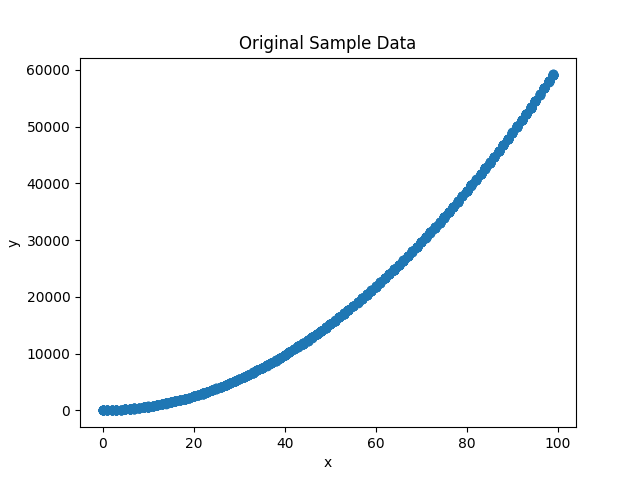
\includegraphics[width=\linewidth]{NonLinear Original.png}
        \caption{Sample Data}
    \end{subfigure}
    \begin{subfigure}{0.5\textwidth}
        \centering
        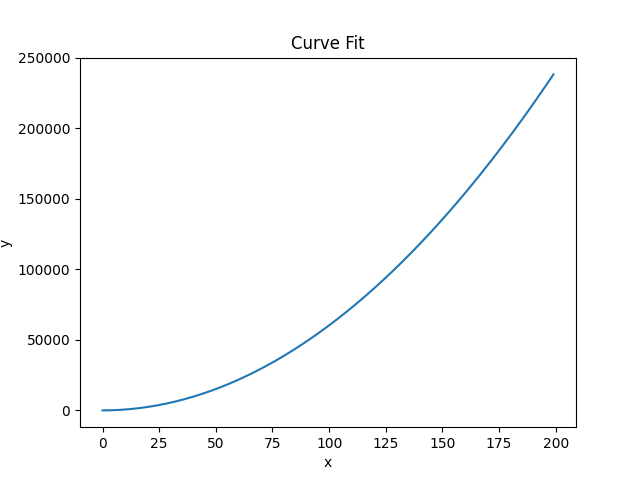
\includegraphics[width=\linewidth]{Non Linear Fit.png}
        \caption{Curve Fitting}
    \end{subfigure}
    \caption{Curve Fitting of Polynomial Regression}
\end{figure}